Os blocos são elementos de fundação de grande rigidez, executados com concreto simples ou ciclópico (portanto, não armado), dimensionado de tal forma que as tensões de tração neles produzidas, sejam absorvidas pelo próprio concreto.

\begin{figure}[htb]
	\begin{center}
	\caption{Nomenclatura das dimensões da base do bloco de fundação.}
    	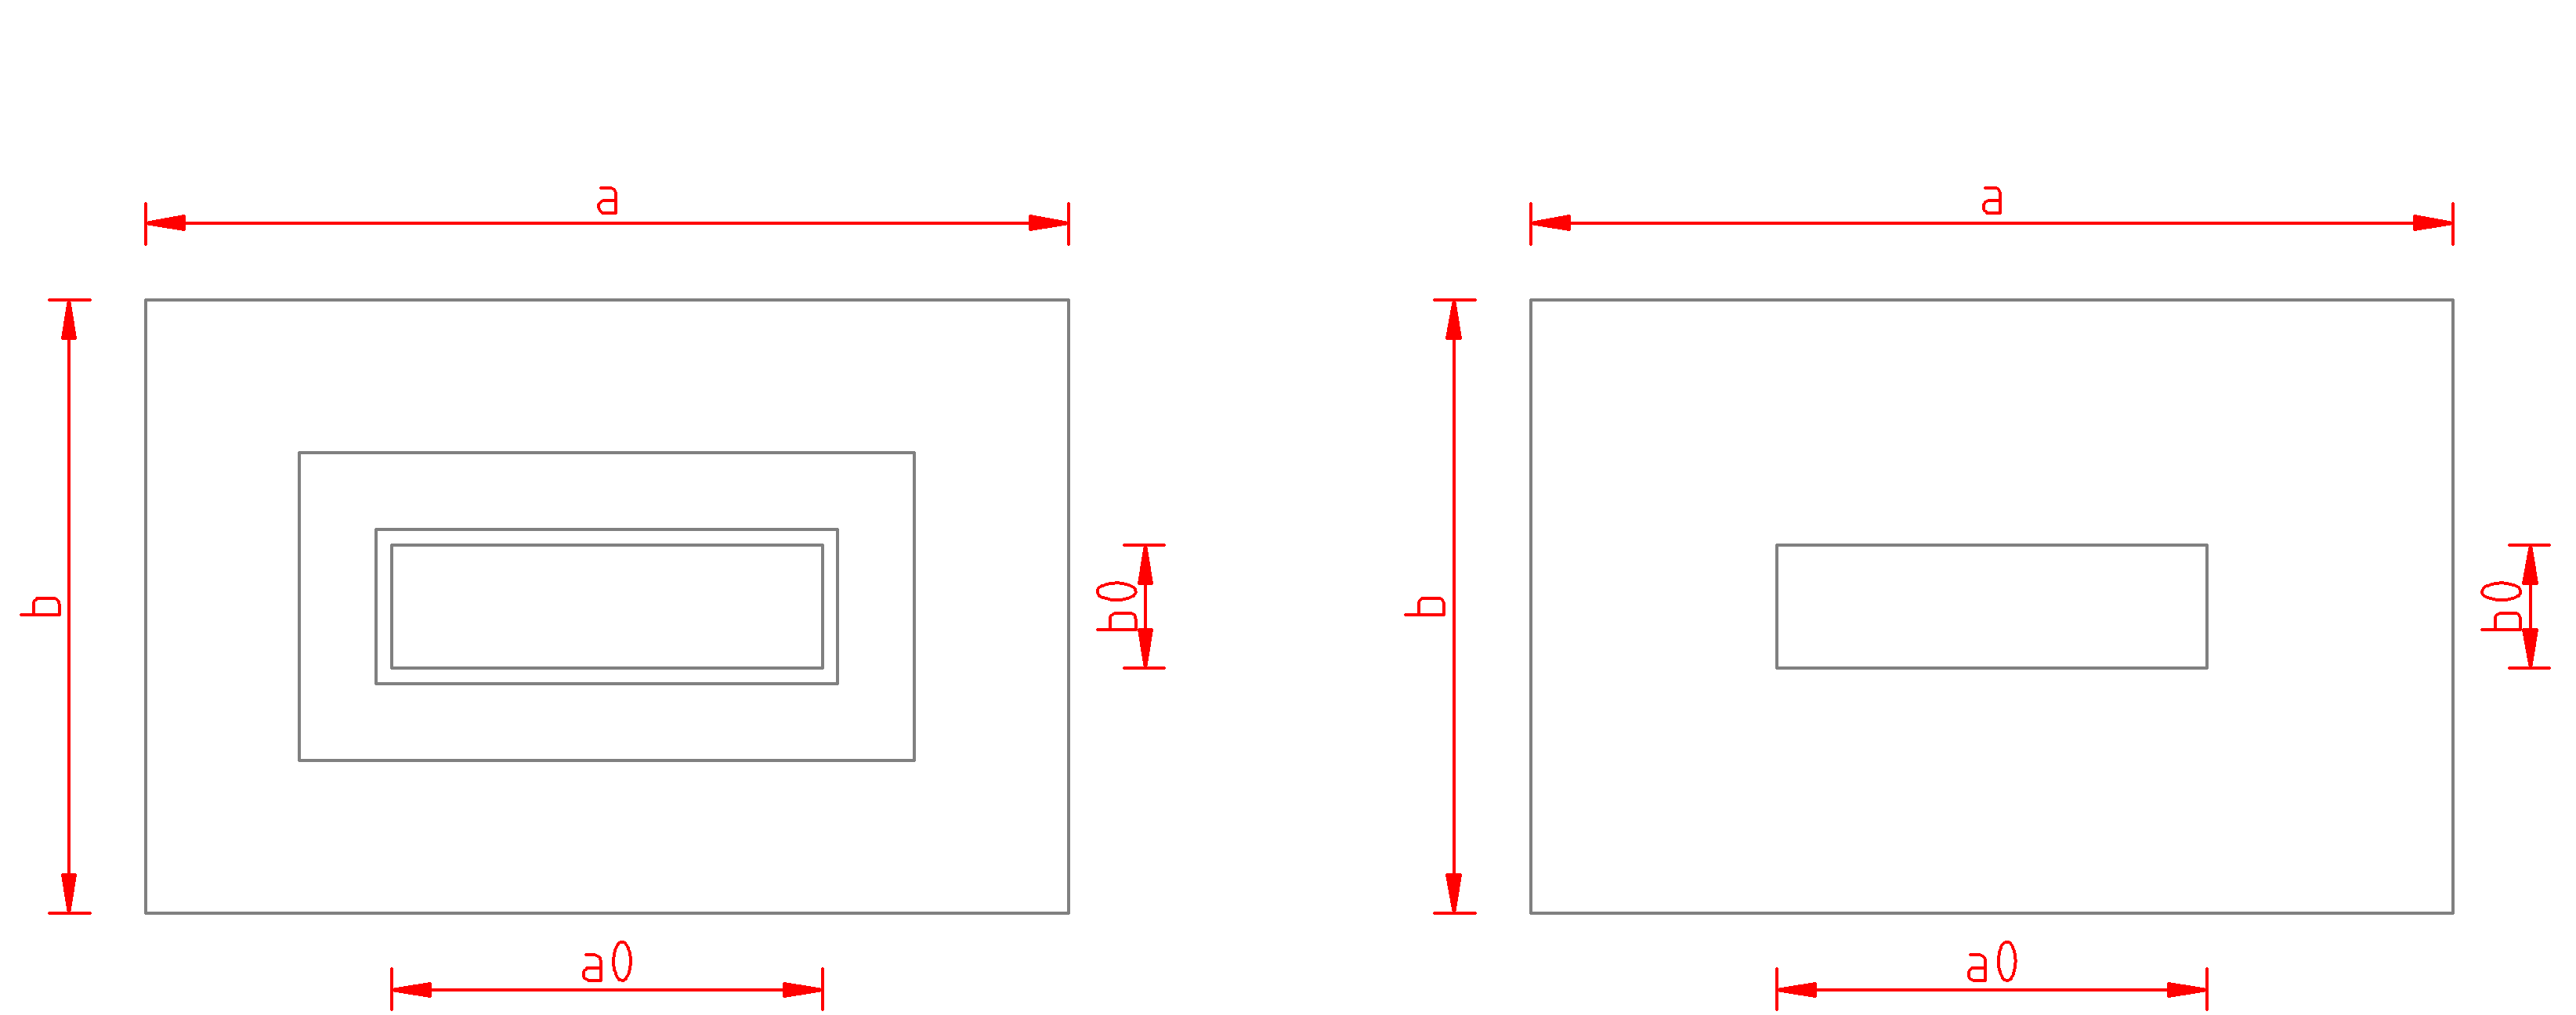
\includegraphics[width=0.9\textwidth]{Fundacoes-rasas-ou-diretas/Imagens/Bloco-de-fundacao-1.png}
	\end{center}
\end{figure}

As equações iniciais são: $$A=a\cdot b$$ $$A=\frac{P}{\sigma_s}$$ $$h=\frac{a-a_0}{2}\cdot \tan{\alpha}$$

\begin{figure}[htb]
	\begin{center}
	\caption{Elementos altura $h$ e ângulo interno $\alpha$ do bloco de fundação. Armadura em azul, pilar em amarelo escuro e o bloco em cinza.}
    	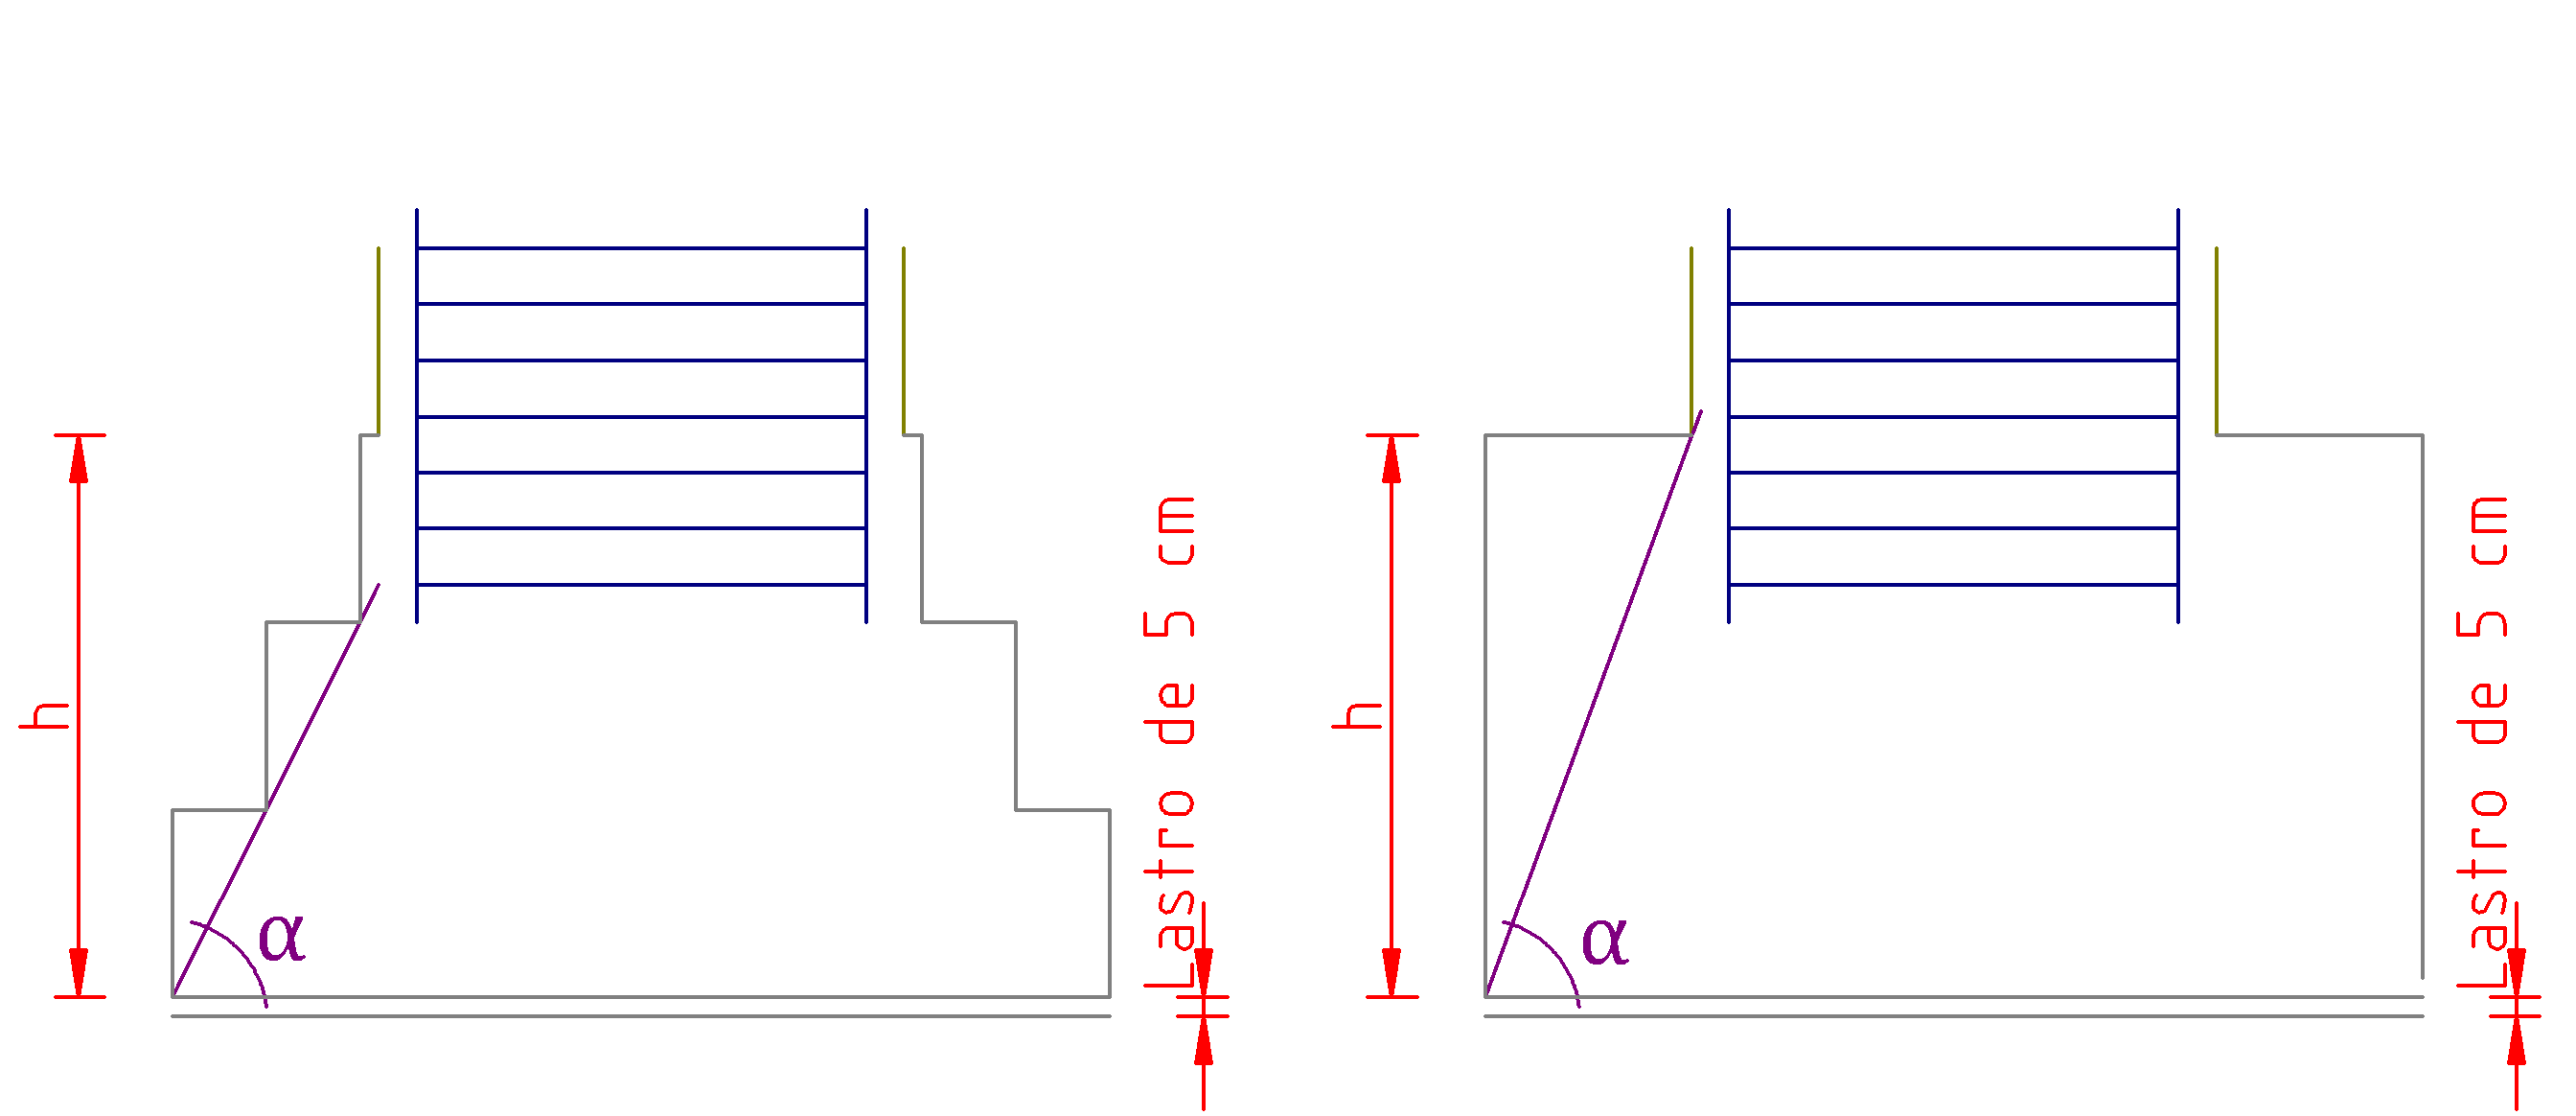
\includegraphics[width=0.9\textwidth]{Fundacoes-rasas-ou-diretas/Imagens/Bloco-de-fundacao-2.png}
	\end{center}
\end{figure}

Onde $a$ é o maior lado do bloco, $b$ é o menor lado do bloco, $a_0$ é o maior lado do pilar, $b_0$ é o menor lado do pilar, $P$ é a carga do pilar, $\sigma_s$ é a tensão admissível do solo, $h$ é a altura do bloco, $\alpha$ é o ângulo interno e $\sigma_t$ é a tensão admissível de tração do concreto.

\begin{figure}[htb]
	\begin{center}
	\caption{Ábaco para encontrar o ângulo interno $\alpha$.}
    	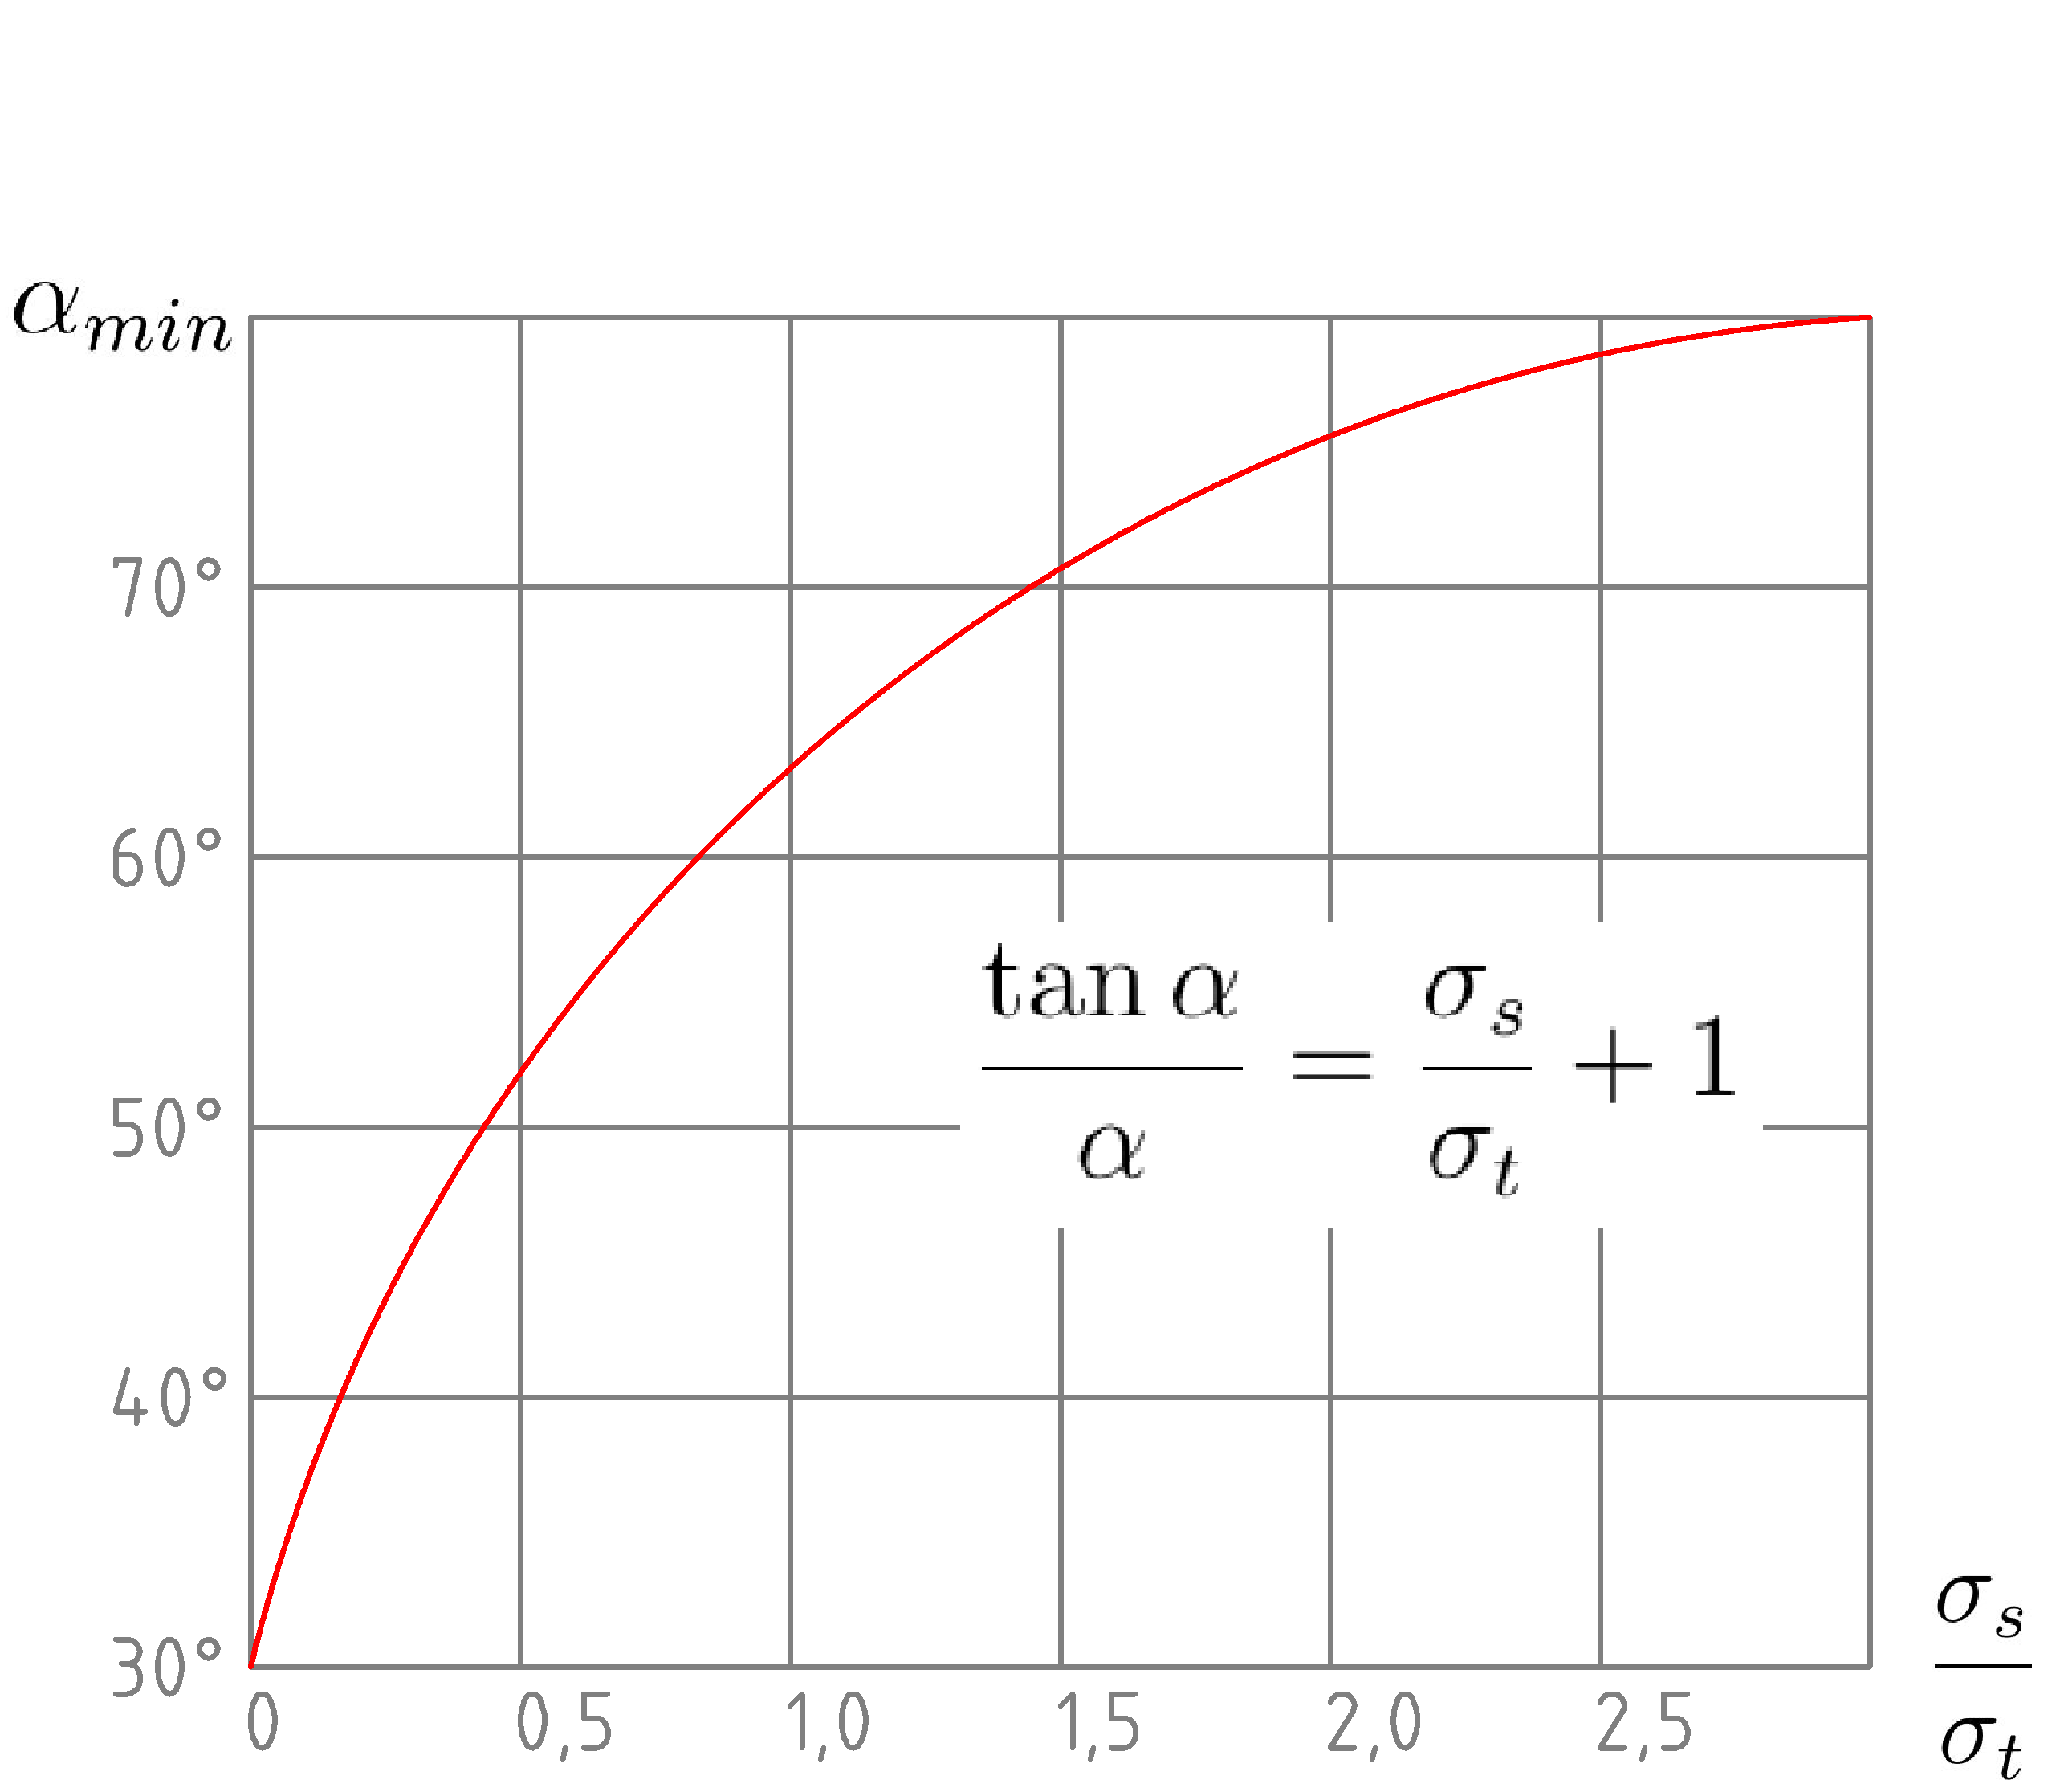
\includegraphics[width=0.5\textwidth]{Fundacoes-rasas-ou-diretas/Imagens/Abaco-bloco-de-fundacao.png}
	\end{center}
\end{figure}

O valor de $\alpha$ é obtido através do ábaco, entrando-se com o valor $\sigma_s/\sigma_t$, em que $\sigma_s$ é a tensão que o bloco aplica ao solo (carga do pilar + peso próprio do bloco, dividido pela área da base) e $\sigma_t$ é a tensão admissível de tração do concreto, que é da ordem de $f_{ck}/25$ e não é recomendável adotar valores superiores a 0,8 $MPa$.

Exemplo: Dimensionar um bloco de fundação sujeito a uma carga de 1700 $kN$, aplicada por um pilar de (35x60) $cm$, executado com concreto com $f_{ck}$ de 15 $MPa$, sobre um solo com taxa igual a 0,4 $MPa$. Desprezar o peso próprio.

O primeiro passo é determinar a área da base, portanto: $$A=\frac{P}{\sigma_s}=\frac{1700\;kN}{0,4\;MPa}=\frac{1700\;kN}{400\;\frac{kN}{m^2}}=4,25\;m^2$$

Como o pilar é retangular, é interessante ter um bloco da mesma forma. Como a $\sqrt{4,25}$ é próxima de 2, estima-se um valor abaixo disso para $b$, a fim de encontrar um valor para $a$ um pouco maior que 2. Portanto, estima-se um $b=1,9\;m$ e o outro lado ($a$) é $4,25\;m^2/1,9\;m\approx 2,25\;m$. Note que o valor dessa divisão foi arredondado para cima, e isso deve ser feito objetivando medidas de 5 em 5 $cm$ (para facilitar a confecção de fôrmas).

Então, determina-se a altura do bloco. Para isso, precisa-se verificar se a tensão admissível de tração do concreto está dentro do limite estabelecido:

$$\sigma_t=\frac{f_{ck}}{25}=\frac{15\;MPa}{25}=0,6\;MPa < 0,8\;MPa$$

O valor está dentro do limite, podemos prosseguir. Agora, deve-se encontrar o ângulo interno do bloco através do ábaco. Primeiramente, verifica-se a seguinte relação: $$\frac{\sigma_s}{\sigma_t}=\frac{0,4\;MPa}{0,6\;MPa}\approx 0,67$$

A relação fornece um $\alpha$ de $\ang{60}$ pelo ábaco. Deve-se verificar a altura em ambas as direções ($a$ e $b$) da peça, como prossegue:

$$h_a=\frac{a-a_0}{2}\cdot \tan{\alpha}=\frac{2,25-0,6}{2}\cdot \tan{\ang{60}}\approx 1,45\;m$$
$$h_b=\frac{b-b_0}{2}\cdot \tan{\alpha}=\frac{1,9-0,35}{2}\cdot \tan{\ang{60}}\approx 1,35\;m$$

Novamente os valores foram arredondados para cima, no mesmo padrão de 5 em 5 $cm$. Adota-se o maior valor de $h$ entre $h_a$ e $h_b$. O bloco de fundação tem $a=2,25\;m$, $b=1,9\;m$ e $h=1,45\;m$.

